\section{Conclusion}

L'étude expose que les formats QIF, IFC et CityGML sont d'excellents containers d'informations pour l'ingénierie de la construction. A contrario, les formats USD et glTF offrent de meilleurs perspectives dans les domaines de la réalité étendue et des environnements immersifs. 

Les graphiques suivants résument, pour chaque format étudié, les 5 points d'analyse que nous avons parcourus : les fonctionnalités techniques offertes par le standard, son adoption dans l'industrie, la complexité de son schéma, la pérennité et la stabilité présumée à date. 

\begin{figure}[!h]
    \centering
    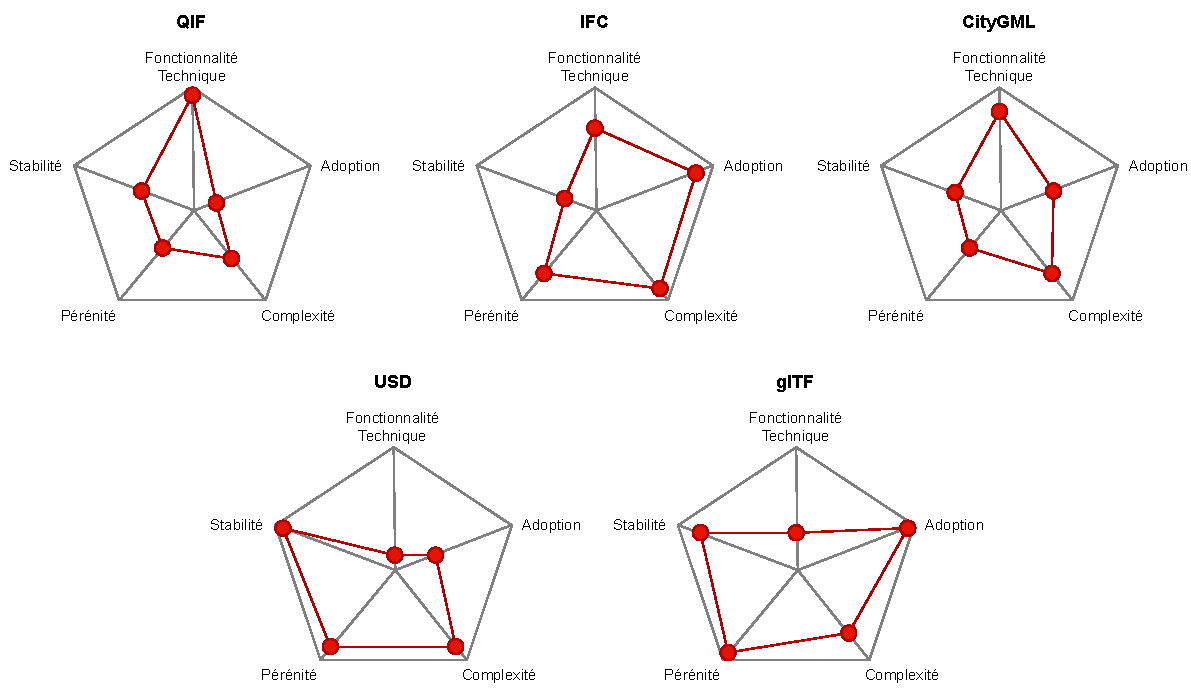
\includegraphics[width=1\linewidth]{imports/3DFiles_Evaluation.pdf}
    \caption{Évaluation globale des formats de fichiers}
    \label{fig:enter-label}
\end{figure}

Les formats de fichiers spécifiques à des domaines d'études tel que le gbXML pour les études énergétiques, le SAF pour l'analyse structurel ou encore l'ILCD pour l'analyse de cycle de vie n'ont pas été étudiés. Cela mériterait une étude complète sur le rapprochement sémantique des différents formats et standards. 

Cependant, constater la complexité des schémas d'informations et l'impossibilité de créer un standard universel de format de fichier 3D (dû aux divergences d'intérêts des utilisateurs finaux) tend à renverser la problématique.

Faut-il nécessairement recourir à l'emploi d'un fichier pour transmettre un ensemble d'information d'un programme à un autre ?
Les containers d'informations sont-ils les seuls à offrir la capacité d'échanger des données entres utilisateurs ?

J'estime qu'il serait plus pertinent de mettre à plat l'ensemble des travaux réalisés par les différentes communautés et consortiums, établir un schéma de donnée évolutif au cas d'usage et le porté sur une technologie conçue spécifiquement pour l'échange d'information à très haute performance : la base de données.

Les systèmes tels que PostgreSQL, MongoDB et autres sont justement prévus pour accueillir un volume considérable d'information. Ils disposent également de toutes les technologies nécessaires au partage de ces données à très haut débit, voir en temps réel, à un ensemble d'utilisateurs. Les API (REST et autres) permettent l'interropérabilité d'à peu près n'importe quel système d'information et application avec des systèmes de gestion de base de données.

Ces technologies sont, par ailleurs, parfaitement compatibles et largement déployés sur le web.


\medskip



